\documentclass{discussion}

\usepackage{amsmath, amsthm, amssymb}
% \usepackage{xcolor, hyperref, cleveref}
\usepackage{mathtools}
% \usepackage{derivative}
\usepackage{graphicx}
\usepackage{tasks}
\usepackage{commands}

\settasks{
    label-width = 1em,
    item-indent = 16pt,
}

\title{MAT 021C Discussion \#1}
\author{Sections B04 and B06}
\date{Fall 2024}

\begin{document}

\section{Review of limits}

\begin{question}
    Let~\(f : \real \to \real\) be a function and~\(x_0 \in \real\) be a point.
    State the definition of~\(\lim_{x\to x_0} f(x)\) and~\(\lim_{x\to \infty} f(x)\).
\end{question}

\vspace{1.4in}

\begin{question}
    Find the following limits or determine that they do not exist:
    \begin{tasks}(2)
        \task \(\displaystyle \lim_{x\to \infty} \left( 5 + \frac{1}{x} \right)\)
        \task \(\displaystyle \lim_{x\to \infty} \frac{\sqrt{5x^2 - 3}}{3x + 2}\)
        \task \(\displaystyle \lim_{x\to \pi/2} \frac{11 (\tan x)^2 + x}{2 (\tan x)^2 + 1}\)
        \task \(\displaystyle \lim_{x \to 0} \frac{\sin x}{x}\)
        \task \(\displaystyle \lim_{x \to \infty} x \sin(1/x)\)
        \task \(\displaystyle \lim_{x \to \infty} \frac{\eu^{x^2}}{x \eu^{x}}\)
    \end{tasks}
\end{question}

\section{Sequential limits}

% Sequential limits are defined analogously to limits of functions.
A sequence \(a_n\) converges if as \(n\) gets large, \(a_n\) gets closer and closer to a real number \(L\).
\begin{center}
    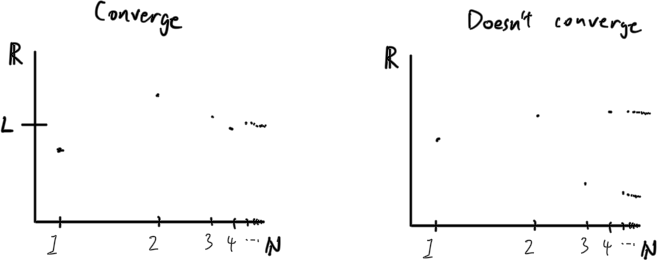
\includegraphics[width=0.5\textwidth]{Sketch 2.png}
\end{center}
% When the natural numbers are written equally spaced, infinity lies infinite far away, and

The formal definition of sequential limits is as follows:
\begin{center}
    \(\displaystyle \lim_{n\to \infty} a_n = L\) if for every \(\epsilon > 0\), there exists an \(N \in \nat\) such that \(\abs{a_n - L} < \epsilon\) for all \(n \geq N\).
\end{center}
\begin{center}
    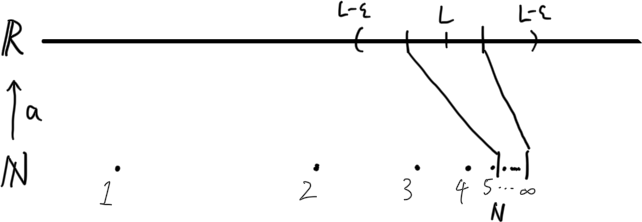
\includegraphics[width=0.5\textwidth]{Sketch.png}
\end{center}

The tools we developed for limits of functions can be used to find limits of sequences thanks to the theorem:
\begin{center}
    If \(\lim_{x\to \infty} f(x) = L\), then \(\lim_{n\to \infty} a_n = L\) where \(a_n = f(n)\).
\end{center}

\begin{question}
    Which of the following sequences converge? If they do, find the limit.
    \begin{tasks}(2)
        \task \(\displaystyle a_n = \frac{3n + 2}{n^2 + 1}\)
        \task \(\displaystyle a_n = \frac{(n+1)! \cdot n^2}{(n+3)!}\)
        \task \(\displaystyle a_n = (-1)^n\)
        \task \(\displaystyle a_n = \cos(2\pi n)\)
        \task \(a_1 = 1\) and \(\displaystyle a_{n+1} = a_n + \left( \frac{1}{n+1} - \frac{1}{n} \right)\)
        \task \(\displaystyle a_n = \frac{4^n}{n}\)
        \task \(\displaystyle a_n = \frac{\ln n}{n}\)
        \task \(\displaystyle a_n = \frac{\ln n}{n^{0.01}}\)
        \task \(\displaystyle a_n = (n + 1) \sin(1/n)\)
        \task \(\displaystyle a_n = n \ln\left( 1 + \frac{1}{n} \right)\)
        \task \(a_1 = 1\) and \(\displaystyle a_{n+1} = \frac{5 + a_n}{2}\)
        \task \(\displaystyle a_n = \frac{n^{100}}{2^{n}}\)
    \end{tasks}
\end{question}

\section{Continuous function theorem}

\begin{question}
    Argue from definitions that if \(\lim_{n\to \infty} a_n = L\) and if \(f\) is a function that is continuous at \(L\) (\textit{i.e.,} \(\lim_{x\to L} f(x) = f(L)\)), then \(\lim_{n\to \infty} f(a_n) = f(L)\).
\end{question}

\vspace{1.2in}

\begin{question}
    Find the limits of the following sequences or determine that they do not exist:
    \begin{tasks}(2)
        \task \(\displaystyle \lim_{n\to \infty} \frac{\sqrt{n + 1}}{\sqrt{n + 3}}\)
        \task \(\displaystyle \lim_{n\to \infty} (\ln n - \ln (n + 1))\)
        \task \(\displaystyle \lim_{n\to \infty} \sqrt[n]{n^2 + 1}\)
        \task \(\displaystyle \lim_{n\to \infty} \left( \frac{n}{n + x} \right)^n\) (any positive real \(x\))
    \end{tasks}
\end{question}

\section{Sandwich theorem}

% TODO Sandwich theorem
Sandwich theorem states that if \(a_n \leq b_n \leq c_n\) for all \(n \geq n_0\), then (assuming the limits exist)
\begin{equation*}
    \lim_{n\to \infty} a_n \leq \lim_{n\to \infty} b_n \leq \lim_{n\to \infty} c_n.
\end{equation*}

\begin{question}
    Find the limits of the following sequences or determine that they do not exist:
    \begin{tasks}(2)
        \task \(\displaystyle \lim_{n\to \infty} \frac{\cos(n)}{n}\)
        \task \(\displaystyle \lim_{n\to \infty} \frac{(-1)^n \cdot n}{1 + n}\)
        \task \(\displaystyle \lim_{n\to \infty} \frac{3^n}{n!}\)
        \task \(\displaystyle \lim_{n\to \infty} \frac{n!}{n^n}\) (hint: compare with \(1/n\))
        \task! \(\displaystyle \lim_{n\to \infty} \frac{2^{(n+1)n}}{n!}\) (hint: \(2^{(n+1)n} = 4^{n} 4^{n-1} \cdots 4^2 4^1\))
    \end{tasks}
\end{question}


\end{document}